\documentclass[skripsi,indonesia]{ugmskripsi}
% Options:
%   skripsi / proposal        (default: skripsi)
%   satuspasi / duaspasi / satusetengahspasi (default: satusetengahspasi)
%   indonesia / inggris       (default: indonesia)

%------------------------------------------------------------
% Metadata Skripsi
%------------------------------------------------------------
\titleind{Perbandingan Prosedur Imperatif Terotomasi Berbasis \texttt{kubectl} dan GitOps dengan ArgoCD untuk Menghadapi Penyimpangan Konfigurasi pada Klaster Kubernetes}
\titleeng{A Comparison of an Automated \texttt{kubectl}-Based Imperative Procedure and ArgoCD GitOps for Addressing Configuration Drift in Kubernetes Clusters}
\fullname{Muhammad Argya Vityasy}
\idnum{23/522547/PA/22475}
\degree{Sarjana}
\gelar{S.Kom.}
\yearsubmit{2026}
\program{Ilmu Komputer}
\dept{Ilmu Komputer dan Elektronika}
\firstsupervisor{Guntur Budi Herwanto, S.Kom., M.Cs.}
\firstexaminer{Dr. techn. Kabul Kurniawan, S.Kom., M.Cs.}
\secondexaminer{Aina Musdholifah, S.Kom., M.Kom., Ph.D.}
\examdate{17 Juni 2026}

%------------------------------------------------------------
% Packages
%------------------------------------------------------------
\usepackage[utf8]{inputenc}
\usepackage{graphicx}
\graphicspath{{figures/}{diagrams/}}
\usepackage{amsmath}
\usepackage{amssymb}
\usepackage{booktabs}
\usepackage{longtable}
\usepackage{tabularx}
\usepackage{multirow}
\usepackage{float}
\usepackage{listings}
\usepackage{xcolor}
\usepackage{hyperref}
\usepackage{url}
\usepackage{xurl}
\usepackage{enumitem}
\usepackage{tikz}
\usetikzlibrary{shapes.geometric,arrows.meta,positioning,fit,backgrounds,calc}

% Code listing style
\lstset{
    basicstyle=\ttfamily\small,
    breaklines=true,
    frame=single,
    numbers=left,
    numberstyle=\tiny,
    keywordstyle=\color{blue},
    commentstyle=\color{gray},
    stringstyle=\color{orange},
    showstringspaces=false,
    tabsize=2
}

% Define YAML language for listings
\lstdefinelanguage{yaml}{
  keywords={true,false,null,y,n},
  sensitive=false,
  comment=[l]{\#},
  morecomment=[s]{/*}{*/},
  morestring=[b]',
  morestring=[b]"
}

% Define Docker language for listings
\lstdefinelanguage{docker}{
  alsoletter={-},
  keywords={FROM,RUN,CMD,LABEL,MAINTAINER,EXPOSE,ENV,ADD,COPY,ENTRYPOINT,VOLUME,USER,WORKDIR,ARG,ONBUILD,STOPSIGNAL,HEALTHCHECK,SHELL},
  sensitive=false,
  comment=[l]{\#},
  morestring=[b]',
  morestring=[b]"
}

%------------------------------------------------------------
% Document Body
%------------------------------------------------------------
\begin{document}
\sloppy

%------------------------------------------------------------
% Daftar Lambang dan Singkatan (DAFTAR SIMBOL)
%------------------------------------------------------------
\nomenclature{GitOps}{Paradigma manajemen \textit{deployment} yang menggunakan repositori Git sebagai \textit{single source of truth} dengan agen \textit{reconciliation} otomatis}
\nomenclature{IaC}{\textit{Infrastructure-as-Code}: praktik mendefinisikan dan mengelola infrastruktur melalui berkas konfigurasi yang diberi versi}
\nomenclature{ArgoCD}{Alat GitOps \textit{pull-based} yang melakukan \textit{continuous reconciliation} terhadap \textit{state} klaster Kubernetes}
\nomenclature{R1}{Metrik konsistensi \textit{deployment}}
\nomenclature{R2}{Metrik waktu deteksi, ketersediaan bukti penyimpangan, dan pemulihan konfigurasi}
\nomenclature{R3}{Metrik \textit{traceability} operasional (deskriptif)}

% Preliminary Pages (Skripsi: lengkap)
\cover
\titlepageind
\approvalpage
\declarepage
\motto
\acknowledment

\preface
Isi Prakata di sini...

\tableofcontents
\addcontentsline{toc}{chapter}{\listtablename}
\listoftables
\addcontentsline{toc}{chapter}{\listfigurename}
\listoffigures
\lambang

\abstractind
Skripsi ini merancang evaluasi empiris atas prosedur imperatif terotomasi berbasis \texttt{kubectl} dan GitOps menggunakan ArgoCD dalam menghadapi penyimpangan konfigurasi pada Kubernetes. Pengujian formal direncanakan pada beban uji multi-service InvenioRDM; surrogat S1 dan S2 hanya digunakan dalam pilot validasi instrumen dan tidak digabungkan dengan data formal. Tujuh intervensi direncanakan, dengan skenario F diperlakukan terpisah sebagai batas visibilitas sumber daya di luar cakupan aplikasi. Metrik yang dirancang mencakup kesetaraan bidang konfigurasi dan kesehatan secara terpisah (R1), waktu deteksi, waktu ketersediaan bukti penyimpangan, dan waktu pemulihan konfigurasi penuh (R2), serta rubrik bukti keterlacakan (R3). Target pengulangan adalah lima run per skenario dan lingkungan untuk R1 serta sepuluh untuk R2; angka ini merupakan target deskriptif, bukan jaminan kecukupan daya. Protokol dan apparatus masih menunggu tinjauan serta validasi, dan data formal belum tersedia. Oleh sebab itu, skripsi ini belum melaporkan hasil komparatif atau kesimpulan empiris.

\vspace{0.5cm}
\noindent\textbf{Kata Kunci:} penyimpangan konfigurasi, Kubernetes, GitOps, otomasi imperatif, evaluasi empiris terkontrol
\endabstractind

\abstracteng
This thesis drafts an empirical evaluation of an automated imperative procedure based on \texttt{kubectl} and GitOps using ArgoCD for configuration drift in Kubernetes. Formal testing is planned on the InvenioRDM multi-service workload; S1 and S2 surrogates are reserved for instrument-validation pilots and will not be pooled with formal data. Seven interventions are planned, with scenario F treated separately as a visibility-boundary case for resources outside the application scope. The measures comprise configuration-field equality and health reported separately (R1), time to detection, availability of verifiable deviation evidence, and full configuration restoration (R2), and an evidence-based traceability rubric (R3). Planned sample targets are five runs per scenario and environment for R1 and ten for R2; these are descriptive targets, not guarantees of statistical power. The protocol and apparatus remain subject to review and validation, and no formal dataset is available. Accordingly, no comparative findings or empirical conclusions are reported in this draft.

\vspace{0.5cm}
\noindent\textbf{Keywords:} configuration drift, Kubernetes, GitOps, automated imperative management, controlled empirical evaluation
\endabstracteng

%------------------------------------------------------------
% Chapters
%------------------------------------------------------------
\chapter{PENDAHULUAN}

\section{Latar Belakang}

Kubernetes mengelola sumber daya aplikasi melalui keadaan yang dideklarasikan dan rekonsiliasi oleh komponen pengendali. Dalam operasi nyata, keadaan aktual dapat berbeda dari deklarasi yang menjadi acuan. Perbedaan ini disebut penyimpangan konfigurasi (\textit{configuration drift}). Penyimpangan perlu dibedakan dari cacat statis: suatu manifest dapat mengandung konfigurasi yang keliru tetapi tetap sama dengan keadaan aktual, sedangkan drift merujuk pada ketidakcocokan antara acuan dan keadaan yang berjalan. Dengan demikian, pengukuran kesetaraan konfigurasi tidak dengan sendirinya menilai apakah nilai konfigurasi tersebut baik atau aman \citep{zhang2026configuration, rahman2023security}.

Pengelolaan deklaratif dapat menggunakan pengendali GitOps untuk membandingkan sumber daya klaster dengan deklarasi di repositori dan mencoba merekonsiliasikannya. Pendekatan imperatif menggunakan perintah untuk mengubah keadaan klaster; perilaku setelah perubahan bergantung pada otomasi dan prosedur yang dipasang. Karena itu, perbandingan empiris perlu menetapkan dengan jelas mekanisme yang dibandingkan. Penelitian ini tidak mengukur kecepatan atau keahlian manusia. Lingkungan pembanding imperatif menggunakan prosedur otomatis berbasis \texttt{kubectl} yang tetap dan terstandarisasi, sementara lingkungan lain menggunakan ArgoCD dengan kebijakan rekonsiliasi yang akan diverifikasi sebelum eksperimen.

Sejumlah penelitian telah mengevaluasi GitOps maupun membandingkannya dengan pendekatan lain. Shrestha dan Ali membahas waktu induksi, penemuan, dan pemulihan drift dalam perbandingan GitOps dengan Ansible \citep{shrestha2024configuration}. Kagganti Nataraja mendeskripsikan perbandingan terkontrol pada Minikube satu node dengan konfigurasi keamanan yang berbeda \citep{kaggantinataraja2025security}. Matubber juga memasukkan pembanding lama yang semi-terotomasi dalam evaluasi infrastruktur Kubernetes \citep{matubber2025managing}. Studi-studi tersebut menunjukkan bahwa evaluasi komparatif telah dilakukan; penelitian ini tidak mengklaim sebagai perbandingan pertama atau menganggap bahwa GitOps pasti lebih unggul. Rincian lingkup dan batas interpretasi studi tersebut dibahas pada Bab II.

Penelitian ini merancang pengukuran per skenario pada beban uji multi-service InvenioRDM. Pengukuran membedakan kesetaraan bidang konfigurasi dari kesehatan layanan, memisahkan waktu deteksi dari ketersediaan bukti yang dapat diverifikasi, dan mengukur pemulihan terhadap kesetaraan inventaris serta bidang yang telah ditetapkan. Keterlacakan dinilai berdasarkan bukti yang tersedia, bukan asumsi bahwa suatu alat selalu menghasilkan jejak lengkap. Skenario F diperlakukan secara terpisah karena menguji batas visibilitas sumber daya di luar cakupan aplikasi, bukan keberhasilan self-heal atas sumber daya terkelola.

Rancangan ini dimaksudkan untuk memperjelas perbedaan operasional antara dua prosedur yang ditetapkan pada konteks eksperimen tertentu. Rekomendasi praktis maupun kesimpulan tentang arah perbedaan hanya dapat dibuat setelah apparatus divalidasi, protokol ditinjau, dan data formal dikumpulkan. Pada draf ini, hasil eksperimen belum tersedia.

\section{Rumusan Masalah}

Penelitian ini diarahkan oleh pertanyaan berikut.

\begin{enumerate}
  \item \textbf{RQ1:} Bagaimana kesetaraan bidang konfigurasi yang ditetapkan dan kesehatan layanan, yang dilaporkan secara terpisah, berubah setelah intervensi dan prosedur koreksi pada prosedur imperatif terotomasi berbasis \texttt{kubectl} dibandingkan dengan GitOps menggunakan ArgoCD?
  \item \textbf{RQ2:} Bagaimana distribusi waktu deteksi, waktu hingga tersedia bukti penyimpangan yang dapat diverifikasi, dan waktu pemulihan konfigurasi penuh berbeda antara kedua prosedur untuk setiap skenario yang dianalisis?
  \item \textbf{RQ3:} Bukti apa yang tersedia untuk merekonstruksi pelaku, objek dan bidang yang berubah, waktu serta urutan kejadian, dan tindakan pemulihan pada masing-masing prosedur?
\end{enumerate}

RQ1 dan RQ2 dijawab per skenario. HPA normal tetap aktif pada kedua lengan; A menjadi kontrol HPA, bukan bukti efikasi ArgoCD memulihkan replika yang diabaikan. A dan uji batas visibilitas F dilaporkan terpisah dari estimasi B--E/G. Tidak adanya OutOfSync bukan waktu deteksi nol. RQ3 bersifat deskriptif dan tidak mengukur waktu identifikasi akar masalah. Penyesuaian tersebut tetap draf untuk tinjauan pemilik dan pembimbing; eksekusi formal dinonaktifkan.

\section{Batasan Masalah}

Ruang lingkup penelitian dibatasi sebagai berikut.

\begin{enumerate}
  \item Perbandingan mencakup satu prosedur imperatif terotomasi berbasis \texttt{kubectl} dan satu implementasi GitOps berbasis ArgoCD. Tidak ada intervensi manusia dalam waktu deteksi atau pemulihan yang diukur; hasil tidak mewakili kecepatan operator atau semua implementasi kedua paradigma.
  \item Beban uji formal direncanakan berupa workload komposit multi-service InvenioRDM pada satu klaster Kubernetes. Komposisi aktual, versi, dan kapasitas lingkungan harus diverifikasi sebelum pengujian. Generalisasi dibatasi pada konfigurasi apparatus yang dilaporkan.
  \item Surrogat S1 dan S2 hanya digunakan pada pilot untuk memvalidasi instrumen dan prosedur. Data pilot tidak menggantikan beban formal, tidak dipool dengan data formal, dan tidak mendukung kesimpulan tentang InvenioRDM.
  \item Intervensi yang direncanakan meliputi perubahan replika, image, ConfigMap, penghapusan sumber daya, patch bidang terkelola, sumber daya pada namespace di luar cakupan aplikasi (F), dan perubahan Secret. F dianalisis sebagai batas visibilitas sumber daya tak terkelola; bukan sebagai skenario self-heal yang diasumsikan.
  \item R1 menilai kesetaraan inventaris dan bidang deklaratif yang ditetapkan dengan aturan sama pada kedua lingkungan; kesehatan dilaporkan terpisah. R2 mencakup waktu deteksi, ketersediaan bukti penyimpangan, dan pemulihan konfigurasi penuh. R3 menggunakan rubrik bukti deskriptif. Nilai Secret tidak dipublikasikan.
  \item Analisis dibatasi pada hasil per skenario. Target jumlah pengulangan merupakan target deskriptif, bukan jaminan kecukupan daya. Data tersensor, kegagalan injeksi, dan kegagalan instrumentasi dilaporkan terpisah; tidak ada nilai hilang yang diganti nol.
\end{enumerate}

\section{Tujuan Penelitian}

Penelitian ini bertujuan merancang dan, setelah protokol disetujui serta apparatus divalidasi, mengevaluasi perbedaan operasional antara prosedur imperatif terotomasi berbasis \texttt{kubectl} dan GitOps berbasis ArgoCD pada beban uji formal multi-service InvenioRDM. Evaluasi mengoperasionalkan RQ1 melalui kesetaraan konfigurasi dan kesehatan yang terpisah, RQ2 melalui waktu deteksi, bukti, serta pemulihan, dan RQ3 melalui rubrik ketersediaan bukti keterlacakan. Tujuan ini tidak menyatakan sebelumnya prosedur mana yang lebih baik.

\section{Manfaat Penelitian}

Jika protokol berhasil divalidasi dan data dikumpulkan, penelitian ini diharapkan dapat:
\begin{enumerate}
  \item memberikan deskripsi empiris yang dibatasi pada workload, skenario, dan konfigurasi yang benar-benar diuji;
  \item mendokumentasikan definisi pengukuran serta aturan penanganan data tersensor agar dapat ditinjau dan direplikasi; dan
  \item menyediakan informasi kontekstual bagi praktisi tanpa mengubah hasil satu apparatus menjadi rekomendasi universal tentang GitOps atau pengelolaan imperatif.
\end{enumerate}

\section{Sistematika Penulisan}

Skripsi ini disusun sebagai berikut:
\begin{itemize}
  \item Bab I menjelaskan latar belakang, rumusan masalah, batasan, tujuan, manfaat, dan sistematika penulisan.
  \item Bab II membahas konsep drift, pendekatan pengelolaan konfigurasi, studi empiris terkait, serta ruang kontribusi yang dibatasi.
  \item Bab III menjelaskan rancangan perbandingan, workload, skenario, definisi metrik, protokol, analisis, dan ancaman validitas.
  \item Bab IV menyediakan struktur pelaporan setup dan bukti untuk R1--R3; hasil empiris hanya dapat diisi setelah eksperimen formal tervalidasi.
  \item Bab V merangkum status kesimpulan, keterbatasan, serta rekomendasi yang dapat ditindaklanjuti setelah hasil tersedia.
\end{itemize}

\chapter{TINJAUAN PUSTAKA}

\section{Penyimpangan Konfigurasi (\textit{Configuration Drift})}

Penyimpangan konfigurasi (\textit{configuration drift}) adalah ketidakcocokan antara keadaan aktual sistem dan keadaan yang ditetapkan sebagai acuan deklaratif \citep{pohjola2025mitigating}. Drift berbeda dari cacat statis: konfigurasi yang tidak aman dapat tetap cocok dengan acuannya, sedangkan perubahan aktual yang tidak cocok dengannya merupakan drift meskipun nilai aktual belum dinilai dampaknya. Penelitian ini mengukur kesetaraan terhadap deklarasi, bukan kebenaran semantik atau keamanan seluruh manifest.

Penelitian empiris oleh \citet{zhang2026configuration} melakukan studi terhadap 719 \textit{defect} konfigurasi dari 2.260 skrip Kubernetes dan mengidentifikasi 15 kategori \textit{defect}, di mana 533 dari 719 \textit{defect} (74,1\%) menyebabkan \textit{crash}, operasi yang salah, atau \textit{outage}. Studi tersebut menegaskan bahwa \textit{misconfiguration} merupakan risiko operasional utama pada Kubernetes. \citet{rahman2023security} menambahkan bahwa \textit{security misconfiguration} pada manifest Kubernetes \textit{open-source} mencakup 11 kategori yang berulang, termasuk \textit{container} yang berjalan sebagai \textit{root}, tanpa \textit{drop capabilities}, dan tanpa \textit{resource limits}. Penelitian menunjukkan bahwa penyimpangan konfigurasi bukan hanya masalah estetika konfigurasi, tetapi ancaman nyata terhadap keandalan dan keamanan layanan.

\citet{pohjola2025mitigating} memberikan kerangka konseptual untuk memahami sumber dan dampak penyimpangan pada sistem \textit{Infrastructure-as-Code} (IaC). Penelitian tersebut mengidentifikasi tiga faktor pendorong utama penyimpangan: (1)~keahlian manusia (\textit{human expertise}) yang tidak konsisten; (2)~tekanan waktu (\textit{time pressure}) yang memicu perubahan cepat dan tidak didokumentasikan; dan (3)~ketiadaan mekanisme deteksi otomatis pada \textit{pipeline deployment}. Meskipun penelitian tersebut tidak beroperasi pada Kubernetes secara eksklusif, prinsip-prinsip yang dikemukakan berlaku umum untuk platform orkestrasi berbasis konfigurasi deklaratif.

\subsection{Faktor yang Menimbulkan Penyimpangan Konfigurasi}

Berdasarkan literatur, faktor-faktor utama yang memperburuk penyimpangan konfigurasi pada Kubernetes meliputi:

\begin{enumerate}
  \item Perubahan langsung pada klaster: Penggunaan \texttt{kubectl\allowbreak{} edit}, \texttt{kubectl\allowbreak{} patch}, atau \texttt{kubectl\allowbreak{} scale} secara langsung tanpa memperbarui repositori \textit{source of truth} \citep{zhang2026configuration}.
  
  \item Prosedur \textit{deployment} yang tidak terdokumentasi: Setiap \textit{operator} dapat memiliki urutan perintah yang berbeda, yang mengakibatkan \textit{state} klaster tidak deterministik \citep{pohjola2025mitigating}.
  
  \item Kurangnya mekanisme \textit{rollback} yang terintegrasi: kemampuan untuk mengembalikan perubahan bergantung pada pencatatan versi, ketersediaan nilai dasar, dan fitur yang dikonfigurasi pada alat pengelolaan \citep{rahman2023security}.
  
  \item Ketiadaan mekanisme deteksi penyimpangan otomatis: Tanpa pemeriksaan berkala antara \textit{state} aktual dan \textit{desired state}, penyimpangan dapat terakumulasi selama periode lama tanpa terdeteksi \citep{zhang2026configuration}.
\end{enumerate}

\section{Terminologi Dasar}

Bagian ini mendefinisikan terminologi kunci yang digunakan dalam penelitian, dengan tujuan membangun dasar konseptual yang konsisten sebelum pembahasan lebih lanjut.

\subsection{Kubernetes dan Orkestrasi Kontainer}
Kubernetes adalah platform \textit{container orchestration} \textit{open-source} yang mengotomasi \textit{deployment}, \textit{scaling}, dan manajemen aplikasi terkemas (\textit{containerized}) \citep{burns2016borg}. Kubernetes awalnya dikembangkan oleh Google berdasarkan pengalaman mengelola sistem \textit{workload} berskala besar di Borg dan Omega, dan kini menjadi standar de facto untuk orkestrasi kontainer di industri \citep{verma2015borg}. Pada Kubernetes, \textit{state} yang diinginkan (\textit{desired state}) dideklarasikan melalui berkas konfigurasi (\textit{manifest}), dan \textit{control plane} bertanggung jawab mencapai dan mempertahankan \textit{state} tersebut.

\subsection{Git dan \textit{Version Control}}
Git adalah sistem \textit{version control} terdistribusi yang merekam setiap perubahan pada berkas beserta metadata (penulis, \textit{timestamp}, pesan \textit{commit}) \citep{chacon2014git}. Dalam konteks GitOps, Git berfungsi sebagai \textit{single source of truth} yang menyimpan deklarasi \textit{state} infrastruktur dan aplikasi, sehingga setiap perubahan dapat dilacak, di-\textit{review}, dan dikembalikan (\textit{rollback}) secara andal.

\subsection{\textit{Continuous Integration} dan \textit{Continuous Deployment}}
\textit{Continuous Integration} (CI) adalah praktik di mana perubahan kode secara otomatis diuji dan digabungkan ke \textit{branch} utama, sementara \textit{Continuous Deployment} (CD) adalah perluasan CI di mana perubahan yang lulus pengujian secara otomatis di-\textit{deploy} ke lingkungan produksi tanpa intervensi manual eksplisit \citep{humble2010continuous}. GitOps merupakan paradigma spesifik di dalam CD yang menggunakan repositori Git sebagai \textit{single source of truth}.

\subsection{\textit{Infrastructure-as-Code} (IaC)}
\textit{Infrastructure-as-Code} (IaC) adalah praktik mendefinisikan dan mengelola infrastruktur melalui berkas konfigurasi yang diberi versi (\textit{versioned}), bukan melalui proses manual \citep{morris2020iac}. IaC memungkinkan \textit{version control}, \textit{code review}, dan reprodusibilitas lingkungan. Dalam konteks Kubernetes, IaC diimplementasikan melalui \textit{manifest} deklaratif (YAML) yang mendefinisikan \textit{desired state} klaster.

\subsection{Paradigma Deklaratif vs Imperatif}
Dalam paradigma imperatif, tindakan pengelolaan dinyatakan sebagai perintah atau urutan tindakan yang mengubah keadaan sistem (\textit{how to achieve the state}). Dalam paradigma deklaratif, keadaan yang diinginkan dinyatakan dan pengendali bertugas mendekatinya (\textit{what state to achieve}) \citep{scott2015plp}. Keduanya dapat diotomasi; perbedaan untuk penelitian ini adalah prosedur koreksi imperatif tetap yang dijalankan melalui \texttt{kubectl} dibandingkan dengan rekonsiliasi ArgoCD.

\section{Manajemen Konfigurasi Infrastruktur}

\textit{Infrastructure state management} mengatur bagaimana keadaan infrastruktur didefinisikan, diterapkan, dan dipertahankan. Pendekatan deklaratif menyimpan keadaan yang diinginkan dalam konfigurasi, sedangkan pendekatan imperatif menyatakan tindakan untuk mengubah keadaan \citep{morris2020iac, limoncelli2018}. Otomasi, pemeriksaan berulang, dan pencatatan dapat tersedia pada kedua pendekatan; karakteristik tersebut perlu ditetapkan pada tingkat implementasi yang dibandingkan.

\section{\textit{Continuous Deployment} dan Paradigma GitOps}

\textit{Continuous Deployment} (CD) adalah praktik dalam ranah DevOps di mana setiap perubahan kode yang lulus pengujian secara otomatis di-\textit{deploy} ke lingkungan produksi tanpa intervensi manual eksplisit \citep{limoncelli2018}. CD merupakan perluasan dari \textit{Continuous Integration} (CI) dan bertujuan meminimalkan waktu antara penulisan kode dan ketersediaannya bagi pengguna akhir. Dalam ekosistem Kubernetes, CD memerlukan mekanisme yang dapat secara andal menyelaraskan perubahan konfigurasi dengan \textit{state} klaster.

GitOps adalah paradigma spesifik di dalam CD yang menggunakan repositori Git sebagai \textit{single source of truth} untuk mendefinisikan \textit{state} infrastruktur dan aplikasi. CNCF GitOps Working Group mendefinisikan empat prinsip OpenGitOps: (1)~sistem dideklarasikan secara deklaratif; (2)~\textit{state} sistem yang diinginkan tersimpan dan diberi versi (\textit{versioned}) dalam Git; (3)~perubahan \textit{state} ditarik (\textit{pulled}) secara otomatis oleh agen \textit{software}; dan (4)~agen \textit{software} secara kontinu mendeteksi dan mengoreksi deviasi dari \textit{state} yang diinginkan \citep{opengitops2021}.

GitOps mendukung pencatatan versi deklarasi melalui Git, peninjauan perubahan, dan penggunaan revisi sebelumnya sebagai acuan pemulihan \citep{yuen2021gitops}. Riwayat Git tidak otomatis merekam perubahan langsung pada klaster; tindakan tersebut memerlukan bukti dari pengendali atau audit API. Pada model \textit{pull-based}, agen di dalam klaster dapat menarik deklarasi tanpa pipeline eksternal menerapkan setiap perubahan ke API klaster, tetapi kebutuhan kredensial dan akses operasional tetap bergantung pada rancangan serta konfigurasi sistem \citep{utami2021analysis}. Klaim adopsi dan manfaat GitOps juga muncul dalam artikel industri CNCF 2025; artikel tersebut dipakai hanya sebagai konteks industri, bukan sebagai bukti \textit{peer-review} \citep{cncf2025gitops}.

\subsection{Performa \textit{Deployment} dan \textit{Anti-Pattern}}

Forsgren dkk. \citep{forsgren2018accelerate} membahas \textit{deployment frequency}, \textit{lead time for changes}, \textit{time to restore service}, dan \textit{change failure rate} sebagai metrik performa pengembangan dan operasi. Metrik organisasi tersebut tidak identik dengan pengukuran eksperimen ini dan tidak dengan sendirinya membuktikan bahwa satu prosedur selalu lebih unggul. Penelitian ini menggunakan konstruk yang lebih terbatas: kesetaraan bidang konfigurasi, waktu deteksi dan pemulihan konfigurasi, serta bukti keterlacakan.

ArgoCD menyediakan pengendali aplikasi yang membandingkan sumber daya teramati dengan deklarasi repositori dan, jika kebijakan serta cakupannya mengizinkan, dapat melakukan sinkronisasi atau koreksi otomatis \citep{argocd2024}. Perilaku aktual bergantung pada konfigurasi aplikasi, izin, ketersediaan pengendali, jenis sumber daya, dan cakupan inventaris. Oleh sebab itu, rekonsiliasi tidak menjamin setiap perubahan akan selalu ditemukan atau dipulihkan.

\section{Dasar Teori: \textit{Reconciliation} dan \textit{Convergence} pada Sistem Deklaratif}

Karakteristik GitOps yang berbeda dari pendekatan imperatif dapat dijelaskan melalui dua prinsip teoretis yang saling berkaitan.

\subsection{\textit{Convergence} Menuju \textit{Desired State}}

Pengendali deklaratif secara berkala membandingkan keadaan aktual dengan keadaan yang diinginkan dan dapat melakukan tindakan korektif sesuai kebijakan yang berlaku \citep{argocd2024}. Keberhasilan konvergensi bukan sifat yang dapat diasumsikan untuk semua sumber daya atau gangguan: hasil dipengaruhi oleh cakupan aplikasi, izin, ketersediaan komponen, konfigurasi sinkronisasi, dan sifat sumber daya.

Perintah imperatif tidak dengan sendirinya menyediakan rekonsiliasi berkelanjutan. Namun, prosedur imperatif dapat diotomasi dengan pemeriksaan berkala dan tindakan koreksi yang telah ditentukan. Karena penelitian ini membandingkan prosedur \texttt{kubectl} terotomasi dengan ArgoCD, bukan respons manusia, perbedaan waktu tidak ditafsirkan sebagai perbedaan kecepatan operator.

\subsection{\textit{Audit Trail} sebagai \textit{Social Control Mechanism}}

Riwayat Git dapat menyediakan metadata dan perubahan deklarasi, sedangkan log pengendali dan audit API dapat memberi bukti tambahan tentang penerapan aktual \citep{opengitops2021}. Riwayat tersebut tidak otomatis membuktikan siapa yang melakukan perubahan pada klaster atau apakah semua tindakan terekam; kelengkapan bergantung pada tata kelola repositori, identitas, konfigurasi audit, dan pengumpulan bukti. Namun, R3 tidak diukur dalam penelitian ini karena audit API server Kubernetes tidak tersedia; keterlacakan dibahas sebagai keterbatasan dan pekerjaan lanjutan, bukan sebagai hasil.

\section{\textit{Runbook} sebagai Standarisasi Prosedur Pemulihan}

\textit{Runbook} adalah dokumen terstandarisasi yang berisi prosedur operasional untuk menanggapi insiden atau melakukan pemulihan (\textit{recovery}) pada sebuah sistem. Dalam ranah operasi TI, \textit{runbook} berfungsi sebagai \textit{playbook} yang mendefinisikan langkah-langkah korektif berurutan berdasarkan jenis insiden, sehingga setiap \textit{operator} yang berbeda mengikuti urutan tindakan yang sama \citep{schlette2024playbook}. Penggunaan \textit{runbook} mengurangi variabilitas akibat keahlian \textit{operator} yang berbeda-beda dan memastikan bahwa keputusan subjektif diminimalkan selama pemulihan.

Dalam rancangan penelitian ini, prosedur imperatif bukan runbook yang dipandu kepada operator. Mode imperatif menggunakan pemeriksa dan korektor otomatis yang tetap, dengan pembandingan deklarasi dan keadaan aktual serta tindakan \texttt{kubectl} yang telah ditetapkan. Mode ini diperoleh dengan menjeda \textit{auto-sync}/\textit{self-heal} ArgoCD pada stack yang sama, lalu memulihkannya. Pilot perlu memverifikasi bahwa prosedur tersebut bekerja tanpa menerima identitas skenario atau label injeksi dan menyimpan bukti yang sama jenisnya dengan evaluator bersama.

\section{Paradigma \textit{Deployment} Alternatif}

Pilihan pengelolaan konfigurasi mencakup rekonsiliasi berbasis tarik, pipeline dorong, alat konfigurasi yang dijalankan sesuai kebutuhan, serta otomasi imperatif khusus. Perbedaan autentikasi, cakupan sumber daya, pencatatan, dan frekuensi eksekusi bergantung pada konfigurasi implementasi; tidak diasumsikan bahwa seluruh pipeline dorong mengekspos kredensial atau bahwa semua alat imperatif tidak memiliki audit. Studi Shrestha dan Ali secara khusus membandingkan GitOps dengan Ansible pada waktu induksi, penemuan, dan pemulihan drift \citep{shrestha2024configuration}.

Penelitian ini membatasi pembanding pada satu prosedur imperatif terotomasi berbasis \texttt{kubectl} dan satu instalasi ArgoCD. Kontras ini tidak merupakan batas atas efek yang berlaku bagi semua alat atau konteks; temuan nantinya hanya berlaku bagi implementasi dan workload yang benar-benar diuji.

\section{Evaluasi Empiris GitOps dan ArgoCD}

Studi terkait telah menguji sejumlah kombinasi alat dan tujuan penelitian. Shrestha dan Ali \citep{shrestha2024configuration} membandingkan GitOps dengan Ansible pada waktu induksi, penemuan, dan pemulihan drift. Kagganti Nataraja \citep{kaggantinataraja2025security} mendeskripsikan perbandingan terkontrol pada klaster Minikube satu node dengan konfigurasi keamanan yang berbeda. Matubber \citep{matubber2025managing} mengevaluasi pengelolaan infrastruktur Kubernetes berbasis GitOps dan mencakup pembanding lama yang semi-terotomasi. Ketiganya menunjukkan bahwa penelitian komparatif atau evaluasi berbasis waktu telah ada; abstrak yang tersedia tidak cukup untuk menyimpulkan ada atau tidaknya uji statistik tertentu.

Utami dan Al Fatta \citep{utami2021analysis} membahas model deployment deklaratif berbasis tarik dibandingkan dengan model berbasis dorong. Paavola \citep{paavola2021managing} membahas pengelolaan beberapa aplikasi Kubernetes menggunakan prinsip GitOps, sedangkan D'Amore \citep{damore2021gitops} mendeskripsikan implementasi ArgoCD pada lingkungan Kubernetes hybrid cloud. Studi tersebut memberi konteks implementasi, tetapi tidak diperlakukan di sini sebagai bukti bahwa salah satu prosedur selalu lebih unggul.

Perbandingan penelitian perlu dibaca sesuai tujuan, alat, lingkungan, konfigurasi, dan hasil yang benar-benar dilaporkan oleh masing-masing sumber. Draf ini tidak menyatakan bahwa penelitian terdahulu tidak terkontrol, tidak menggunakan statistik, atau tidak memiliki baseline apabila pernyataan itu tidak dapat dipastikan dari abstrak yang tersedia.

\section{Metode Eksperimental Terkontrol pada Riset Sistem}

Evaluasi empiris pada riset sistem dan infrastruktur memerlukan desain yang memitigasi ancaman terhadap validitas \citep{wohlin2012experimentation}. Penelitian ini merupakan studi kasus komparatif terkontrol: satu kasus diamati pada kondisi dasar, satu intervensi, dan kondisi pascaintervensi, dengan dua mode pengelolaan yang dijalankan berurutan \citep{runeson2009case}. \citet{limoncelli2018} menjelaskan bahwa penelitian sistem harus membangun lingkungan yang dapat direproduksi, mengendalikan variabel pengganggu, dan mendefinisikan metrik yang jelas sebelum menyimpulkan hubungan kausal.

Rancangan penelitian ini menetapkan mode imperatif terotomasi berbasis \texttt{kubectl} dan mode GitOps berbasis ArgoCD sebagai dua perlakuan pada satu stack. Kesetaraan \textit{workload}, nilai dasar, inventaris pengukuran, dan prosedur injeksi direncanakan untuk mengurangi perbedaan yang tidak relevan. Karena kedua implementasi dapat berbeda dalam lebih dari satu komponen teknis dan tidak ada isolasi penuh, hasil tidak langsung diatribusikan sebagai efek universal paradigma; interpretasinya dibatasi pada prosedur dan kasus yang benar-benar diuji \citep{wohlin2012experimentation}.

Analisis yang direncanakan bersifat per skenario dan eksploratif. Ringkasan distribusi, jumlah observasi lengkap dan tersensor, serta ukuran efek dan interval kepercayaan dilaporkan bersama-sama; uji komparatif hanya digunakan jika asumsi dan struktur data mendukungnya. Sampel formal 15 pengulangan per skenario per mode (210 run) tidak dianggap sebagai bukti daya statistik yang memadai \citep{dyba2006power,kitchenham2024small}. Rincian definisi operasional dan batas interpretasi terdapat pada Bab III.

\section{Klasifikasi Beban Uji (\textit{Workload})}

Aplikasi yang dijalankan pada klaster Kubernetes dapat dikelompokkan ke dalam beberapa kelas \textit{workload} berdasarkan karakteristik arsitektur dan manajemen \textit{state} \citep{siddiqui2023microservices, aghili2024workload}:

\begin{enumerate}
  \item \textit{Workload} web tanpa state (\textit{stateless web microservice}): Layanan yang tidak menyimpan \textit{state} secara internal, sehingga setiap permintaan dapat dilayani oleh instans mana pun. Contoh: server HTTP sederhana, \textit{API gateway}.
  
  \item \textit{Workload} berbasis data yang menyimpan \textit{state} (\textit{stateful data service}): Layanan yang menyimpan \textit{state} secara persisten, seperti \textit{database} relasional, \textit{search engine}, atau \textit{object storage}. \textit{Workload} kelas ini memerlukan urutan \textit{deployment} dan penanganan penyimpangan yang lebih kompleks.
  
  \item \textit{Workload} komposit multi-service: Aplikasi yang terdiri atas banyak komponen yang saling bergantung, mencakup kombinasi kelas 1 dan 2 beserta komponen infrastruktur (\textit{ingress}, TLS, \textit{secrets}, \textit{monitoring}, \textit{backup}, kebijakan keamanan). Kelas \textit{workload} ini memiliki kompleksitas dependensi tertinggi dan paling rentan terhadap penyimpangan konfigurasi akibat banyaknya komponen yang harus diselaraskan.
\end{enumerate}

Pengujian formal dalam rancangan ini menggunakan beban uji komposit multi-service InvenioRDM pada satu stack produksi-like. Inventaris dan komponen aktual harus dicatat dari konfigurasi yang divalidasi sebelum eksperimen; jumlah komponen yang pernah disebut sebagai target belum diverifikasi. Beban uji merupakan konteks pengukuran, bukan dasar untuk menggeneralisasi hasil ke seluruh \textit{workload} multi-service. Surrogat S1/S2 historis/offline tidak dipakai dalam desain formal dan tidak memperluas sampel formal.

\section{Ruang Kontribusi Penelitian}

Studi komparatif mengenai GitOps dan pengelolaan konfigurasi telah ada, termasuk evaluasi terhadap Ansible, pengujian terkontrol pada Minikube, dan pengukuran yang mencakup \textit{baseline} semi-terotomasi. Karena itu, penelitian ini tidak berangkat dari klaim bahwa perbandingan terdahulu tidak ada atau bahwa keunggulan GitOps telah terbukti secara universal.

Kontribusi yang diklaim bersifat terbatas dan dapat diperiksa: (1)~perbandingan empiris pada \textit{deployment} InvenioRDM multi-service nyata, bukan \textit{workload} sintetis; (2)~dua mode yang dijalankan berurutan pada satu stack produksi-like, dengan mode imperatif didefinisikan sebagai penjedaan ArgoCD ditambah pemeriksa/\textit{runbook} \texttt{kubectl}, sehingga perbandingan tidak memerlukan stack kembar; (3)~pengukuran R1/R2 yang dapat direproduksi dengan kepemilikan HPA, \textit{drift} Service F yang dilaporkan terpisah, dan kasus G yang dipisahkan dari efikasi; serta (4)~bukti batas bahwa hasilnya berlaku untuk kasus dan apparatus yang diuji, bukan klaim superioritas GitOps universal. R3 tidak diukur karena audit API server tidak tersedia dan dibahas sebagai keterbatasan serta pekerjaan lanjutan.

Hasil yang kelak diperoleh hanya dapat menjawab pertanyaan pada skenario, \textit{workload}, konfigurasi, dan resolusi instrumentasi yang benar-benar diuji. Besaran maupun arah perbedaan belum dapat dipastikan sebelum pengumpulan serta analisis data formal.

\chapter{METODE PENELITIAN}

\section{Deskripsi Umum dan Status Protokol}

Penelitian ini dirancang sebagai evaluasi empiris terkontrol atas dua prosedur pengelolaan \textit{deployment}: prosedur imperatif terotomasi berbasis \texttt{kubectl} dan GitOps berbasis ArgoCD. Pertanyaan yang dituju ialah bagaimana kedua prosedur tersebut berbeda pada konsistensi konfigurasi, waktu deteksi, ketersediaan bukti penyimpangan, pemulihan konfigurasi, dan keterlacakan untuk skenario yang ditetapkan. Estimand dibatasi pada selisih hasil antarprosedur dalam konteks beban uji multi-service InvenioRDM dan apparatus eksperimen yang kelak diverifikasi; estimand ini bukan efek universal seluruh paradigma imperatif atau GitOps.

Naskah ini memuat rancangan protokol, bukan laporan pelaksanaan. Protokol masih memerlukan tinjauan pembimbing, dan apparatus eksperimen yang tersedia belum divalidasi untuk mengimplementasikan seluruh definisi operasional di bawah. Versi perangkat lunak, kesiapan klaster, inventaris sumber daya formal, dan data eksperimen belum ditetapkan atau diverifikasi dalam naskah ini. Karena itu, uraian rencana tidak boleh dibaca sebagai bukti bahwa eksperimen telah dilaksanakan.

\section{Rancangan Perbandingan}

Pengendalian kondisi awal, pengulangan, pencatatan penyimpangan protokol, dan pembatasan inferensi mengikuti prinsip evaluasi empiris perangkat lunak \citep{wohlin2012experimentation}. Karena pengujian memakai lingkungan yang dibangun secara sengaja pada satu klaster, rancangan tidak dianggap sebagai penugasan acak klaster dari suatu populasi \citep{cook1979quasi}.

Unit analisis adalah satu injeksi penyimpangan yang diterima pada satu lingkungan dalam satu pengulangan. Lingkungan A menggunakan otomasi imperatif tetap: pemeriksa berkala membandingkan keadaan aktual dengan inventaris dan nilai yang diinginkan, menyimpan perbedaan yang teramati, lalu menjalankan prosedur koreksi \texttt{kubectl} yang telah ditentukan. Lingkungan B menggunakan ArgoCD dengan rekonsiliasi otomatis terhadap deklarasi Git. Tidak ada operator yang menunggu, mengetik, atau memilih tindakan korektif selama pengukuran; waktu respons manusia maupun tingkat keahlian operator bukan variabel penelitian.

Kedua lingkungan memakai beban uji, nilai dasar, definisi bidang yang diperiksa, serta prosedur injeksi dan pengukuran yang setara. Injeksi dilakukan satu per satu, bukan serentak, dan urutan lingkungan serta skenario diacak dalam blok pengujian setelah kondisi dasar dipulihkan. Pengendali koreksi hanya menerima keadaan aktual dan deklarasi yang diperlukan untuk membandingkannya; identitas skenario tidak diteruskan sebagai label, termasuk pada skenario Secret. Rancangan ini membandingkan dua implementasi operasional yang telah ditentukan, bukan mengisolasi seluruh faktor yang mungkin membedakan setiap produk atau organisasi.

\begin{figure}[H]
  \centering
  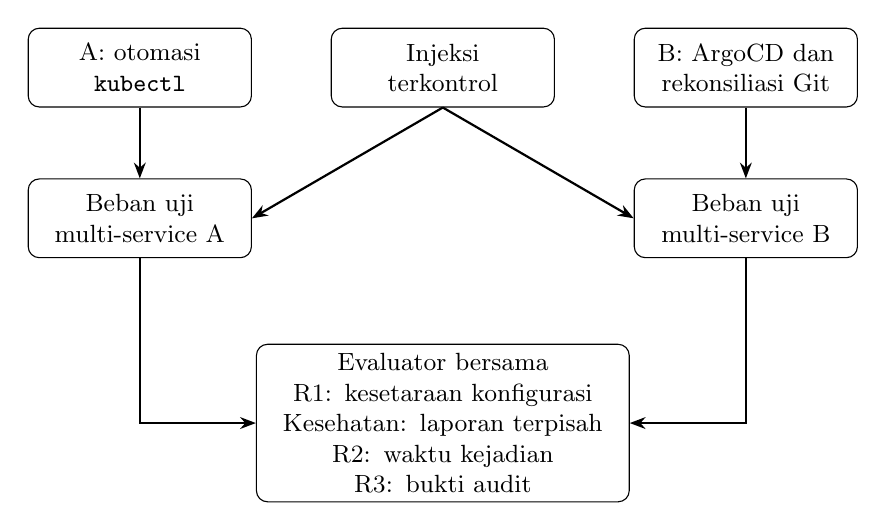
\begin{tikzpicture}[
    box/.style={draw, rounded corners, align=center, text width=2.6cm, minimum height=10mm, font=\small},
    flow/.style={-{Stealth[length=2mm]}, thick},
    node distance=9mm and 5mm
  ]
    \node[box] (inject) {Injeksi\\terkontrol};
    \node[box, left=10mm of inject] (kubectl) {A: otomasi\\\texttt{kubectl}};
    \node[box, right=10mm of inject] (argocd) {B: ArgoCD dan\\rekonsiliasi Git};
    \node[box, below=of kubectl] (worka) {Beban uji\\multi-service A};
    \node[box, below=of argocd] (workb) {Beban uji\\multi-service B};
    \node[box, below=30mm of inject, text width=4.5cm] (measure) {Evaluator bersama\\R1: kesetaraan konfigurasi\\Kesehatan: laporan terpisah\\R2: waktu kejadian\\R3: bukti audit};
    \draw[flow] (inject.south) -- (worka.east);
    \draw[flow] (inject.south) -- (workb.west);
    \draw[flow] (kubectl) -- (worka);
    \draw[flow] (argocd) -- (workb);
    \draw[flow] (worka.south) |- (measure.west);
    \draw[flow] (workb.south) |- (measure.east);
  \end{tikzpicture}
  \caption{Rancangan perbandingan dua prosedur otomatis dengan evaluator dan definisi metrik yang sama.}
  \label{fig:arsitektur-eksperimen}
\end{figure}

Gambar~\ref{fig:arsitektur-eksperimen} menunjukkan bahwa injeksi, mekanisme pengelolaan, dan evaluator merupakan bagian yang dibedakan secara eksplisit. Hasil hanya akan ditafsirkan untuk konfigurasi apparatus yang benar-benar dicatat saat eksperimen.

\section{Alur Penelitian}

Tahapan yang direncanakan meliputi peninjauan protokol, validasi instrumen melalui uji pendahuluan, pengujian formal, dan analisis per skenario. Uji pendahuluan menggunakan surrogat sederhana S1 dan S2 hanya untuk memeriksa kelayakan injeksi, pencatatan waktu, pemeriksa kesetaraan, dan prosedur reset. Data S1/S2 tidak masuk ke sampel formal dan tidak digunakan untuk menyimpulkan perilaku InvenioRDM.

\begin{figure}[H]
  \centering
  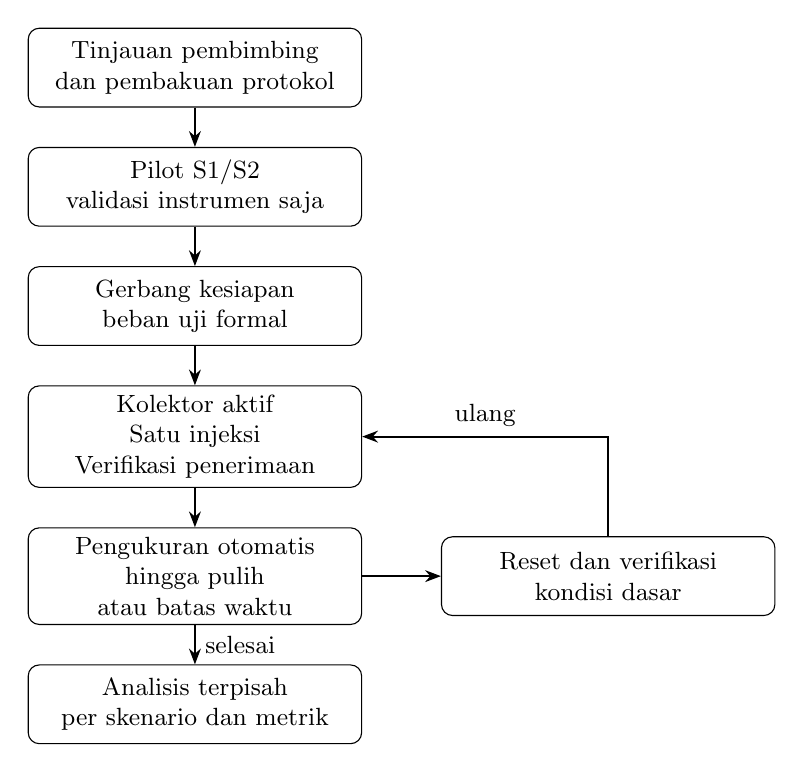
\begin{tikzpicture}[
    process-box/.style={draw, rounded corners, align=center, text width=4cm, minimum height=10mm, font=\small},
    flow/.style={-{Stealth[length=2mm]}, thick},
    node distance=5mm and 10mm
  ]
    \node[process-box] (review) {Tinjauan pembimbing\\dan pembakuan protokol};
    \node[process-box, below=of review] (pilot) {Pilot S1/S2\\validasi instrumen saja};
    \node[process-box, below=of pilot] (ready) {Gerbang kesiapan\\beban uji formal};
    \node[process-box, below=of ready] (inject) {Kolektor aktif\\Satu injeksi\\Verifikasi penerimaan};
    \node[process-box, below=of inject] (measure) {Pengukuran otomatis\\hingga pulih atau batas waktu};
    \node[process-box, right=of measure] (reset) {Reset dan verifikasi\\kondisi dasar};
    \node[process-box, below=of measure] (analyze) {Analisis terpisah\\per skenario dan metrik};
    \draw[flow] (review) -- (pilot);
    \draw[flow] (pilot) -- (ready);
    \draw[flow] (ready) -- (inject);
    \draw[flow] (inject) -- (measure);
    \draw[flow] (measure) -- (reset);
    \draw[flow] (reset.north) |- node[pos=0.75, above, font=\small] {ulang} (inject.east);
    \draw[flow] (measure) -- node[right, font=\small] {selesai} (analyze);
  \end{tikzpicture}
  \caption{Bagan alir protokol, dengan pilot dipisahkan dari pengulangan formal.}
  \label{fig:bagan-alir-eksperimen}
\end{figure}

Gambar~\ref{fig:bagan-alir-eksperimen} menempatkan validasi sebelum pengumpulan data formal dan mensyaratkan pemulihan kondisi dasar di antara pengulangan. Tidak ada jeda buatan setelah injeksi untuk menunggu respons manusia.

\section{Beban Uji dan Lingkungan}

Pengujian formal direncanakan menggunakan beban uji komposit multi-service InvenioRDM dengan sasaran sedikitnya 16 komponen aplikasi dan infrastruktur pendukung sesuai ruang lingkup proposal. Sasaran tersebut bukan jumlah komponen yang telah diverifikasi. Inventaris formal mencakup seluruh sumber daya dalam manifest yang disetujui untuk kedua lingkungan; daftar komponen, batas pengelolaan, dan versinya akan dicatat dari artefak yang benar-benar digunakan. Komponen infrastruktur bersama harus dibedakan dari sumber daya yang menjadi sasaran injeksi agar isolasi kedua lingkungan dapat diperiksa. S1/S2 merupakan surrogat pilot, bukan pengganti beban formal, dan tidak boleh digabungkan ke hasil atau analisis formal.

Rancangan membatasi pengujian pada satu klaster Kubernetes dan satu implementasi GitOps, ArgoCD. Spesifikasi serta versi aktual klaster, node, komponen beban uji, dan ArgoCD harus diverifikasi dan dicatat sebelum pengujian; nilai yang pernah disebut sebagai sasaran pada draf sebelumnya belum menjadi fakta eksperimen. Dua lingkungan perlu memiliki inventaris dan nilai dasar yang sebanding serta terisolasi agar koreksi satu lingkungan tidak mengubah lingkungan lain.

\subsection{Gerbang Kesiapan}

Pengulangan formal hanya dimulai setelah seluruh prasyarat berikut diperiksa dan dicatat: (1) manifest dan inventaris sumber daya formal telah dibekukan; (2) kedua lingkungan berada pada kesetaraan nilai yang ditetapkan dan kesehatan layanan telah memenuhi kriteria kesiapan; (3) auto-sync, self-heal, cakupan aplikasi, dan kebijakan prune ArgoCD telah diverifikasi sesuai rancangan; (4) pemeriksa imperatif, pengumpul bukti, serta pembanding bidang telah lulus uji pilot; (5) jam pencatat waktu tersinkronisasi; dan (6) tidak ada pengujian atau perubahan lain yang berlangsung pada lingkup sumber daya yang diamati. Ambang kesehatan, batas beban, interval ArgoCD, serta batas waktu pengamatan akan dibakukan setelah pilot dan tinjauan pembimbing; naskah ini tidak menyatakan nilai aktualnya.

Jika prasyarat gagal, injeksi tidak dimulai. Gangguan setelah injeksi dicatat sebagai kejadian pengujian, bukan dihapus tanpa jejak. Kriteria penghentian, nilai batas waktu, dan aturan pengulangan harus ditetapkan sebelum data formal dikumpulkan.

\section{Intervensi dan Skenario}

Intervensi adalah satu perubahan terkontrol terhadap keadaan sumber daya dalam satu pengulangan. Skenario A--E dan G menyasar sumber daya yang termasuk inventaris aplikasi; skenario F menguji batas visibilitas untuk sumber daya di luar cakupan aplikasi dan dianalisis terpisah.

\begin{table}[H]
  \centering
  \small
  \caption{Skenario intervensi yang direncanakan}
  \label{tab:skenario-intervensi}
  \begin{tabularx}{\textwidth}{|c|>{\raggedright\arraybackslash}p{3.3cm}|X|}
    \hline
    Skenario & Intervensi & Batas interpretasi \\
    \hline
    A & Mengubah jumlah replika Deployment terkelola & Perubahan terhadap nilai dasar pada inventaris aplikasi \\
    \hline
    B & Mengubah referensi image Deployment terkelola & Perubahan bidang yang telah ditetapkan dalam skema pengukuran \\
    \hline
    C & Mengubah bidang ConfigMap terkelola & Tidak mengubah deklarasi sumber kebenaran \\
    \hline
    D & Menghapus sumber daya terkelola & Pemulihan dinilai terhadap inventaris dan nilai dasar \\
    \hline
    E & Mengubah bidang sumber daya terkelola melalui patch & Hanya bidang yang telah ditetapkan yang dinilai \\
    \hline
    F & Membuat atau menerapkan sumber daya pada namespace di luar cakupan aplikasi & Kasus batas visibilitas sumber daya tak terkelola; bukan keberhasilan atau kegagalan self-heal yang diasumsikan \\
    \hline
    G & Mengubah data Secret terkelola di luar deklarasi & Perbandingan dilakukan tanpa menyimpan atau menampilkan nilai Secret \\
    \hline
  \end{tabularx}
\end{table}

Pada skenario F, sumber daya di luar inventaris aplikasi tidak dianggap sebagai drift terkelola yang wajib dipulihkan ArgoCD. Pengamatan dibatasi pada apakah batas cakupan dan pencatatan inventaris membuat keberadaan sumber daya tersebut terlihat. Hasil F dilaporkan tersendiri dan tidak digabungkan ke estimasi utama A--E dan G.

\section{Definisi Variabel dan Metrik}

\subsection{R1: Kesetaraan Konfigurasi dan Kesehatan}

Kesetaraan konfigurasi dinilai menggunakan aturan yang sama pada kedua lingkungan. Sebelum eksperimen, skema bidang yang diperiksa dan inventaris sumber daya yang diharapkan dibekukan. Bidang dinamis yang tidak relevan bagi deklarasi dikecualikan secara eksplisit. Untuk setiap sumber daya yang diharapkan, sumber daya dinyatakan cocok jika keberadaannya sesuai inventaris dan semua bidang terpilih sama dengan nilai yang diinginkan.

\[
  R1_{eq} = \frac{\text{jumlah sumber daya terkelola yang cocok}}{\text{jumlah sumber daya dalam inventaris yang diharapkan}} \times 100\%.
\]

Evaluator menghitung $R1_{eq}$ dari pembacaan keadaan aktual dan inventaris yang sama bentuknya untuk kedua lengan; status \textit{Synced} ArgoCD bukan pengganti aturan kesetaraan tersebut. Nilai dicatat pada kondisi dasar, pengamatan pertama setelah injeksi, dan setelah prosedur koreksi. Jika koreksi mendahului pengamatan pascainjeksi, kondisi sesaat tersebut ditandai tidak teramati; kondisi drift tidak direkonstruksi seolah-olah telah diukur. Nilai Secret dibandingkan secara aman di memori; nilai mentah maupun hash yang dapat digunakan untuk menebak isinya tidak ditulis ke log, gambar, atau laporan.

Kesehatan layanan dilaporkan sebagai hasil terpisah berdasarkan kriteria kesiapan yang ditetapkan sebelum eksperimen, misalnya kondisi kesiapan Pod dan status layanan yang memang tersedia pada workload. Kesehatan tidak dimasukkan ke pembilang kesetaraan konfigurasi. Sumber daya ekstra di luar inventaris, termasuk F, dilaporkan terpisah dan tidak mengubah penyebut R1.

\subsection{R2: Deteksi, Ketersediaan Bukti, dan Pemulihan}

Semua waktu berasal dari satu kolektor pada host pencatat. Setiap kejadian diberi waktu jam monotonik dalam detik dengan pecahan desimal serta cap waktu UTC untuk audit; durasi dihitung dari jam monotonik, bukan dari selisih jam dinding. Pengamatan diaktifkan sebelum injeksi dan berlangsung pada interval nominal satu detik. Cap waktu adalah waktu pengamatan pertama, bukan waktu kejadian yang diinterpolasi; interval aktual dan jeda polling dicatat. Interval ini merupakan resolusi pengamatan yang direncanakan dan harus divalidasi pada pilot. Interval pemeriksa imperatif dan jadwal rekonsiliasi ArgoCD dicatat tersendiri dari interval evaluator, dibekukan sebelum pengujian formal, dan tidak disesuaikan setelah hasil terlihat.

\begin{itemize}
  \item $t_0$: waktu kolektor mulai mengirim permintaan injeksi ke Kubernetes API. Waktu penerimaan respons API juga dicatat sebagai $t_a$, sehingga $t_a-t_0$ mendokumentasikan latensi permintaan. Injeksi diterima hanya jika operasi API berhasil dan objek respons atau pembacaan balik memverifikasi perubahan bidang sasaran. Durasi sejak $t_0$ mencakup latensi permintaan, bukan semata-mata waktu respons setelah perubahan tersimpan. Injeksi gagal atau tidak terverifikasi dicatat sebagai kegagalan injeksi, bukan sebagai waktu deteksi nol.
  \item $t_d$: waktu pertama mekanisme pengelolaan memberi sinyal deteksi berdasarkan perbedaan dari nilai yang diinginkan. Pada A, sinyal berasal dari pemeriksa imperatif; pada B, dari status perbedaan ArgoCD yang relevan. Tidak ada sinyal skenario tersembunyi yang diberikan kepada mekanisme tersebut.
  \item $t_e$: waktu pertama bukti dari mekanisme pengelolaan tersimpan dan mengidentifikasi sumber daya serta bidang yang berbeda terhadap acuan. Bukti harus dapat diperiksa ulang tanpa memakai label injeksi yang tersembunyi; untuk Secret cukup dicatat identitas bidang dan hasil ketidakcocokan, bukan isinya. Kriteria ini hanya mengukur bukti deviasi, bukan kelengkapan seluruh unsur R3 atau identifikasi penyebab. $t_e$ dapat sama dengan $t_d$, tetapi keduanya tetap dicatat terpisah. Pengumpulan bukti tidak menunda koreksi pada salah satu lingkungan.
  \item $t_r$: waktu pengamatan pertama ketika inventaris dan seluruh bidang R1 kembali cocok dengan nilai yang diinginkan, dengan kecocokan dikonfirmasi pada pembacaan berikutnya. Waktu yang dilaporkan tetap waktu pengamatan pertama; konfirmasi hanya mencegah keadaan sesaat dinyatakan pulih. Kesehatan layanan dilaporkan terpisah.
\end{itemize}

Durasi utama adalah waktu deteksi $t_d-t_0$, waktu ketersediaan bukti $t_e-t_0$, dan waktu pemulihan konfigurasi penuh $t_r-t_0$. Selang dari deteksi ke bukti ($t_e-t_d$) dapat ditampilkan sebagai rincian tambahan. $t_r$ berarti pemulihan kesetaraan inventaris dan bidang yang diukur, bukan klaim bahwa seluruh layanan sehat atau tidak mengalami dampak lain.

Sinyal deteksi A berasal dari pemeriksaan otomatis terhadap keadaan aktual; setelah sinyal muncul, prosedur koreksi tetap menerapkan deklarasi yang diinginkan menggunakan tindakan \texttt{kubectl} yang telah ditetapkan. B menggunakan rekonsiliasi ArgoCD. Kedua prosedur berjalan otomatis tanpa waktu reaksi manusia dan tanpa jeda buatan. Keputusan koreksi menggunakan hasil perbandingan umum, bukan label A--G yang disembunyikan dari responden.

\subsection{R3: Rubrik Bukti Keterlacakan}

R3 dinilai deskriptif untuk setiap pengulangan dengan rubrik yang sama, bukan diasumsikan lengkap karena salah satu alat digunakan. Penilai mencatat ada, sebagian, atau tidak ada bukti untuk unsur berikut.

\begin{table}[H]
  \centering
  \small
  \caption{Rubrik penilaian bukti R3}
  \label{tab:rubrik-r3}
  \begin{tabularx}{\textwidth}{|>{\raggedright\arraybackslash}p{2.5cm}|X|>{\raggedright\arraybackslash}p{4cm}|}
    \hline
    Unsur & Kriteria bukti & Contoh sumber yang diperiksa \\
    \hline
    Pelaku & Identitas aktor atau akun layanan yang melakukan perubahan dapat ditelusuri & Log audit API Kubernetes; log eksekusi otomatis \\
    \hline
    Objek dan perubahan & Objek serta bidang yang berubah dapat ditentukan tanpa menampilkan data sensitif & Diff ArgoCD yang telah disanitasi; catatan perbandingan imperatif \\
    \hline
    Waktu dan urutan & Waktu serta urutan injeksi, deteksi, dan pemulihan dapat direkonstruksi & Cap waktu kolektor; log audit; metadata Git \\
    \hline
    Tindakan dan hasil & Tindakan koreksi dan hasil verifikasinya dapat dikaitkan dengan pengulangan & Log koreksi; riwayat sinkronisasi; pembacaan verifikasi \\
    \hline
  \end{tabularx}
\end{table}

Rubrik ini mengukur ketersediaan bukti perubahan dan tindakan. Rubrik tidak meminta penilai menyimpulkan penyebab kausal atau akar masalah dari sebuah diff. Data audit dapat memuat identitas sensitif; pelaporan hanya menggunakan informasi minimum yang telah disanitasi.

\section{Protokol Pengulangan dan Penanganan Kegagalan}

Satu pengulangan mengikuti urutan berikut:
\begin{enumerate}
  \item Periksa gerbang kesiapan dan simpan bukti kondisi dasar, inventaris, kesehatan, serta status instrumentasi.
  \item Aktifkan koleksi sinyal deteksi, bukti, kesetaraan, dan kesehatan sebelum mengirim injeksi; pastikan mekanisme pengelolaan juga telah aktif. Jalankan hanya satu skenario pada satu lingkungan. Catat $t_0$, respons API pada $t_a$, dan verifikasi penerimaan injeksi tanpa menambahkan label atau identitas skenario ke sumber daya yang diamati.
  \item Pertahankan koleksi berkala satu detik tanpa menyisipkan waktu tunggu agar manusia bereaksi atau agar drift bertahan selama durasi tertentu. Jika perubahan diterima tetapi sinyal singkat tidak teramati, laporkan keterbatasan observasi tanpa menganggap deteksi terjadi pada waktu nol.
  \item Lanjutkan sampai pemulihan terkonfirmasi atau batas waktu pengamatan yang telah dibakukan tercapai. Simpan semua kejadian, jeda polling, kesalahan API, serta status penghentian.
  \item Pulihkan kondisi dasar, verifikasi kesetaraan inventaris dan kesehatan, lalu baru mulai pengulangan berikutnya.
\end{enumerate}

Batas waktu maksimum pengamatan harus ditentukan dan dibekukan setelah pilot serta tinjauan pembimbing, sebelum pengumpulan formal. Tidak ada nilai batas waktu yang diklaim telah diuji dalam draf ini. Jika sinyal deteksi, bukti, atau pemulihan belum terjadi saat batas itu tercapai, hasil masing-masing ditandai tersensor kanan pada batas tersebut; waktu hilang tidak diganti nol dan pengulangan tidak dikeluarkan hanya karena pemulihannya gagal. Kegagalan injeksi, kegagalan instrumentasi, gangguan infrastruktur, dan tidak terjadinya deteksi merupakan kategori berbeda. Setiap kategori, jumlah pengulangan terdampak, alasan, serta aturan pengulangan yang telah disetujui dilaporkan.

Run dengan respons injeksi sukses tetapi tanpa bukti bahwa perubahan bidang sasaran pernah diterima tidak menjadi hasil nol; run ditandai sebagai injeksi tidak valid dan dicatat. Jika perubahan diterima tetapi mekanisme tidak mendeteksinya sampai batas pengamatan, itu merupakan hasil deteksi tersensor, bukan kegagalan instrumen. Jika kolektor atau sumber data gagal sehingga status tidak dapat ditentukan, run ditandai kegagalan instrumentasi dan tidak ditafsirkan sebagai deteksi terlewat. Skenario F tetap diklasifikasikan sebagai pengamatan batas visibilitas dan tidak dinilai dengan asumsi pemulihan otomatis.

\section{Pengulangan dan Analisis Data}

Target rancangan adalah $n=5$ pengulangan per skenario dan per lingkungan untuk R1 serta $n=10$ untuk R2. Angka tersebut merupakan target deskriptif yang direncanakan, bukan hasil analisis daya dan bukan jaminan kecukupan daya untuk setiap skenario. Pengulangan R3 mengikuti pengumpulan bukti pada run yang sama dan dianalisis secara deskriptif. S1/S2 tidak dihitung dalam target ini. Skenario F dilaporkan tersendiri dan tidak dimasukkan ke ringkasan utama skenario drift terkelola A--E dan G.

Hasil disajikan per skenario dan per lingkungan: jumlah run direncanakan, jumlah injeksi valid, jumlah kejadian teramati dan tersensor, ringkasan distribusi waktu, proporsi pemulihan pada batas pengamatan, R1, kesehatan terpisah, serta rubrik R3. Nilai mentah yang hilang tidak diimputasi sebagai nol. Observasi yang tersensor tidak diam-diam dibuang agar hanya run yang berhasil pulih yang dibandingkan. Jika penyensoran terjadi, ringkasan dan uji yang tidak memperhitungkan penyensoran tidak ditafsirkan sebagai perbandingan lengkap; analisis komparatif untuk hasil tersebut harus ditetapkan sebelum melihat hasil, atau dilaporkan secara deskriptif tanpa klaim inferensial.

Untuk hasil waktu yang teramati lengkap, rencana analisis eksploratif menggunakan uji Mann--Whitney U dua sisi apabila asumsi independensi pengulangan terpenuhi. Cliff's $\delta$ ditetapkan sebagai ukuran efek utama agar pilihan ukuran efek tidak bergantung pada arah hasil yang terlihat. Distribusi, median, rentang, dan ukuran sampel yang benar-benar tersedia tetap dilaporkan. Jika nilai $p$ digunakan, ambang nominalnya adalah $\alpha=0{,}05$ dengan penyesuaian Holm untuk keluarga perbandingan waktu yang dibakukan sebelum pengumpulan formal. Definisi keluarga uji dan pemenuhan independensi harus ditinjau bersama pembimbing sebelum protokol dibekukan; tidak ada klaim konfirmatoris dari draf ini. Penggabungan lintas skenario tidak menjadi analisis utama karena bentuk dan dampak intervensinya berbeda. R1, kesehatan, R3, dan kasus F dilaporkan deskriptif; tidak ada hasil signifikansi atau besar efek yang dinyatakan sebelum data dikumpulkan.

\section{Ancaman terhadap Validitas dan Keterbatasan Rancangan}

Validitas internal dapat terancam oleh perbedaan beban klaster dari waktu ke waktu, perubahan konfigurasi selain intervensi, ketidaksetaraan inventaris, serta perbedaan jadwal rekonsiliasi. Isolasi namespace, nilai dasar yang dibekukan, urutan pengujian yang diacak, pencatatan keadaan, dan gerbang kesiapan dirancang untuk mengurangi ancaman tersebut, tetapi tidak menjamin bahwa satu-satunya perbedaan adalah paradigma abstrak. Perbandingan tetap mengikutsertakan perbedaan implementasi yang melekat pada pemeriksa/korektor \texttt{kubectl} dan ArgoCD.

Validitas konstruk dibatasi oleh tujuh skenario yang dipilih, definisi bidang yang dibandingkan, interval polling, batas waktu, kriteria kesehatan, dan rubrik bukti. Pengamatan polling memberikan waktu deteksi pada resolusi instrumen, bukan waktu kejadian kontinu yang persis. Skenario F menguji batas inventaris dan tidak dapat digeneralisasi sebagai pengukuran self-healing untuk sumber daya terkelola.

Validitas eksternal dibatasi pada satu klaster, satu beban uji formal multi-service InvenioRDM, satu alat GitOps, serta konfigurasi dan versi yang kelak benar-benar digunakan. Pilot S1/S2 tidak memperluas cakupan inferensi. Tidak ada kesimpulan yang dapat digeneralisasi ke semua aplikasi, klaster, atau alat GitOps dari rancangan ini saja.

Reliabilitas bergantung pada konsistensi kolektor, sinkronisasi jam, cakupan log, dan kemampuan mengulang reset. Sebelum data formal dikumpulkan, keberhasilan pencatatan, pembandingan Secret tanpa kebocoran, deteksi kegagalan, serta aturan pemulihan dan penyensoran harus diuji. Sampai gerbang tersebut dipenuhi, hasil eksperimen belum tersedia dan protokol tetap berstatus draf.

\chapter{HASIL DAN ANALISIS}

\section{Status Data dan Provenans}

Pada draf ini belum tersedia dataset eksperimen formal yang tervalidasi. Apparatus belum diuji terhadap keseluruhan protokol pada Bab III dan protokol masih menunggu tinjauan pembimbing. Oleh karena itu, bagian ini mendefinisikan informasi yang perlu dilaporkan, tetapi tidak menyajikan angka, uji statistik, ukuran efek, atau kesimpulan komparatif.

Sebelum pengisian hasil, dokumentasikan konfigurasi klaster yang benar-benar digunakan, versi Kubernetes dan ArgoCD, cakupan aplikasi, kebijakan auto-sync/self-heal/prune, manifest serta inventaris formal, interval polling aktual, sinkronisasi jam, dan kriteria kesiapan. Nilai yang pernah disebut sebagai target pada draf sebelumnya bukan hasil verifikasi. Laporkan pula setiap penyimpangan protokol, kegagalan kesiapan, dan perubahan apparatus.

Pengujian formal direncanakan pada workload multi-service InvenioRDM. Pilot S1/S2 hanya dapat mendukung laporan validasi instrumen dan prosedur; hasilnya tidak dipool atau ditafsirkan sebagai hasil formal. Identitas sensitif dan seluruh nilai Secret harus disanitasi dari log, tabel, gambar, serta lampiran.

\section{Format Pelaporan E1: Kesetaraan dan Kesehatan (R1)}

Kesetaraan inventaris dan bidang yang ditetapkan dilaporkan terpisah dari kesehatan layanan. Evaluator yang sama digunakan pada kedua lingkungan. Tabel~\ref{tab:hasil-r1} merupakan skema pelaporan, bukan hasil; isinya menunggu pengumpulan data formal.

\begin{table}[H]
  \centering
  \small
  \caption{Skema hasil R1 per skenario dan lingkungan}
  \label{tab:hasil-r1}
  \begin{tabularx}{\textwidth}{|c|c|X|X|}
    \hline
    Skenario & Lingkungan & Kesetaraan konfigurasi: dasar / pascainjeksi / pascapemulihan & Kesehatan layanan pada pengamatan terkait \\
    \hline
    A--E, G & kubectl / ArgoCD & Belum tersedia & Belum tersedia \\
    \hline
    F & kubectl / ArgoCD & Tidak termasuk hasil utama R1; dicatat sebagai batas cakupan & Dilaporkan terpisah jika relevan \\
    \hline
  \end{tabularx}
\end{table}

\section{Format Pelaporan E2: Waktu (R2)}

Untuk setiap skenario dan lingkungan, hasil kelak mencantumkan target run, jumlah injeksi terverifikasi, jumlah waktu teramati dan tersensor, serta durasi deteksi ($t_d-t_0$), ketersediaan bukti ($t_e-t_0$), dan pemulihan konfigurasi penuh ($t_r-t_0$). Nilai waktu dihitung dari cap waktu kolektor dan tidak diinterpolasi melewati jeda polling.

\begin{table}[H]
  \centering
  \small
  \caption{Skema hasil R2 per skenario dan lingkungan}
  \label{tab:hasil-r2}
  \begin{tabularx}{\textwidth}{|c|c|X|X|}
    \hline
    Skenario & Lingkungan & Run valid / tersensor dan alasan & Distribusi durasi: deteksi / bukti / pemulihan \\
    \hline
    A--E, G & kubectl / ArgoCD & Belum tersedia & Belum tersedia \\
    \hline
    F & kubectl / ArgoCD & Dilaporkan sebagai pengamatan batas visibilitas & Tidak menjadi hasil pemulihan drift terkelola \\
    \hline
  \end{tabularx}
\end{table}

Run tanpa deteksi, bukti, atau pemulihan sampai batas pengamatan akan tetap tampak sebagai tersensor kanan dan disertai jumlahnya. Kegagalan injeksi dan kegagalan instrumentasi dicatat terpisah dari kejadian mekanisme tidak mendeteksi. Run dengan pemulihan tidak lengkap tidak dihilangkan hanya untuk membentuk distribusi waktu yang lebih menguntungkan.

\section{Format Pelaporan E3: Keterlacakan (R3)}

Penilaian R3 akan disajikan berdasarkan rubrik yang sama untuk pelaku, objek/bidang perubahan, waktu/urutan, dan tindakan/hasil pemulihan. Setiap unsur diberi status ada, sebagian, atau tidak ada dengan rujukan ke bukti yang telah disanitasi. Tidak ada nilai hasil yang tersedia pada draf ini. Rubrik tidak menghasilkan waktu identifikasi akar masalah dan tidak digunakan untuk membuat klaim tentang penyebab kausal.

\section{Rencana Analisis Komparatif}

Ringkasan dan perbandingan dilakukan per skenario, bukan dengan menggabungkan semua intervensi menjadi satu angka. Target pengulangan R1 adalah lima run per skenario dan lingkungan, sedangkan R2 sepuluh run; keduanya merupakan target deskriptif dan belum dibuktikan cukup untuk mendeteksi efek pada setiap skenario. Statistik deskriptif, jumlah run valid, kejadian tersensor, serta ukuran efek yang sesuai harus dilaporkan bersama hasil.

Uji Mann--Whitney U hanya dapat dipertimbangkan secara eksploratif untuk hasil waktu yang teramati lengkap jika unit analisis dan asumsi independensi terpenuhi. Jika terdapat penyensoran, hasil uji yang mengabaikannya tidak boleh ditafsirkan sebagai perbandingan lengkap; metode untuk data tersensor harus dibakukan sebelum melihat hasil atau hasil dilaporkan deskriptif. Tidak ada nilai $p$, ukuran efek, ataupun interpretasi arah perbedaan yang dapat dituliskan sebelum pengumpulan serta analisis data formal.

\section{Batas Interpretasi}

RQ1 hanya dapat dijawab terhadap inventaris dan bidang yang ditetapkan; kesetaraan bukan bukti bahwa konfigurasi benar secara semantik. RQ2 membedakan sinyal deteksi, tersedianya bukti yang dapat diverifikasi, dan kembalinya konfigurasi ke keadaan yang diinginkan; kesehatan layanan tetap dilaporkan sebagai dimensi terpisah. RQ3 mendeskripsikan bukti yang tersedia, bukan akar masalah.

Skenario F tidak dianggap sebagai keberhasilan self-heal maupun sebagai kegagalan ketika sumber daya berada di luar cakupan aplikasi ArgoCD. F harus dibahas sebagai pengujian batas visibilitas sumber daya tak terkelola. Kesimpulan tentangnya tidak digabungkan dengan skenario A--E dan G.

Sampai data formal tersedia, tidak dapat dinyatakan prosedur mana yang lebih konsisten, lebih cepat, atau lebih terlacak. Kondisi ini merupakan batas bukti draf, bukan hasil eksperimen negatif dan bukan bukti bahwa instrumentasi gagal.

\chapter{KESIMPULAN DAN SARAN}

\section{Kesimpulan}

Naskah ini telah merumuskan rancangan untuk membandingkan prosedur imperatif terotomasi berbasis \texttt{kubectl} dengan GitOps berbasis ArgoCD pada workload formal multi-service InvenioRDM. Rancangan membedakan kesetaraan konfigurasi dari kesehatan layanan, memisahkan waktu deteksi, ketersediaan bukti, dan pemulihan konfigurasi penuh, serta menggunakan rubrik deskriptif untuk keterlacakan.

Kesimpulan empiris untuk setiap pertanyaan penelitian belum dapat ditarik:
\begin{enumerate}
  \item \textbf{RQ1:} Perbedaan kesetaraan konfigurasi dan kesehatan layanan belum diketahui karena data formal belum tersedia.
  \item \textbf{RQ2:} Perbedaan waktu deteksi, ketersediaan bukti penyimpangan, dan pemulihan konfigurasi belum diketahui. Tidak ada hasil waktu yang dapat diisi dengan asumsi atau angka sintetik.
  \item \textbf{RQ3:} Perbandingan kelengkapan bukti keterlacakan belum dapat dinilai sebelum log dan artefak formal diperiksa.
\end{enumerate}

Dengan demikian, draf ini tidak menyimpulkan efektivitas, keunggulan, atau kelayakan adopsi salah satu prosedur. Skenario F kelak harus dilaporkan terpisah sebagai batas visibilitas sumber daya tak terkelola, bukan sebagai bukti keberhasilan atau kegagalan rekonsiliasi.

\section{Saran}

Sebelum pengujian formal, protokol perlu ditinjau pembimbing, lalu apparatus harus divalidasi terhadap definisi penerimaan injeksi, skema inventaris dan bidang, keselamatan pencatatan Secret, interval polling, timestamp, kriteria kesehatan, batas waktu, serta mekanisme reset. Pilot S1/S2 hanya digunakan untuk memeriksa instrumen; setelah pilot, konfigurasi formal multi-service InvenioRDM tetap harus diuji sesuai rancangan dan tidak boleh digantikan oleh surrogat.

Pengumpulan data berikutnya sebaiknya mencatat konfigurasi serta versi yang benar-benar digunakan, mempertahankan semua kategori kegagalan dan penyensoran, melaporkan hasil per skenario, dan menyimpan bukti yang telah disanitasi. Klaim komparatif perlu dibatasi pada prosedur, workload, klaster, dan resolusi instrumen yang diuji. Penelitian lanjutan dapat menguji workload, ukuran klaster, atau implementasi GitOps lain, tetapi perlu membakukan definisi metrik dan membedakan setiap pembanding secara eksplisit.

\section{Keterbatasan Penelitian}

Keterbatasan yang telah melekat pada rancangan ini meliputi penggunaan satu klaster, satu workload formal, dan satu implementasi GitOps; hasilnya tidak otomatis berlaku bagi konteks lain. Prosedur imperatif yang diuji adalah satu otomasi \texttt{kubectl} tertentu, sehingga tidak mewakili semua cara kerja imperatif. Interval polling membatasi ketelitian waktu kejadian, dan target pengulangan bukan jaminan daya statistik per skenario.

Skenario F berada di luar cakupan sumber daya terkelola dan hanya menguji batas visibilitas. Pengukuran kesetaraan tidak menilai apakah konfigurasi yang diinginkan aman atau benar secara semantik. Selain itu, versi apparatus, inventaris formal, batas waktu pengamatan, serta kriteria kesehatan belum diverifikasi dalam draf ini. Protokol juga belum memperoleh tinjauan pembimbing dan kemampuan apparatus untuk menjalankannya belum divalidasi. Seluruh keterbatasan tersebut perlu dipertimbangkan sebelum hasil empiris tersedia atau rekomendasi praktis dirumuskan.


%------------------------------------------------------------
% Bibliography
%------------------------------------------------------------
\bibliography{references}

%------------------------------------------------------------
% Appendices
%------------------------------------------------------------
\appendix
\chapter{LAMPIRAN A}

Lampiran ini disiapkan untuk artefak yang akan dipublikasikan setelah protokol ditinjau, apparatus divalidasi, dan pengumpulan data formal dilakukan. Pada draf ini, skrip, konfigurasi aktual, dan dataset tervalidasi belum dilampirkan. Ketiadaan artefak tersebut tidak menunjukkan bahwa pengujian telah berhasil atau gagal.

\section{Artefak Eksperimen yang Direncanakan}

Lampiran versi akhir dapat memuat sumber pemeriksa dan korektor imperatif berbasis \texttt{kubectl}, konfigurasi aplikasi ArgoCD, manifest dan inventaris workload formal, skema kolektor, serta prosedur pemulihan nilai dasar. Setiap artefak perlu diberi versi dan dikaitkan dengan konfigurasi aktual eksperimen. Materi pilot S1/S2 harus dipisahkan dari artefak dan data pengujian formal.

\section{Skema Data dan Perlindungan Informasi}

Skema log formal perlu menyimpan pengenal run, lingkungan, skenario pada berkas metadata terpisah dari masukan pengendali, status penerimaan injeksi, cap waktu monotonik dalam detik dan UTC untuk $t_0$, $t_a$, $t_d$, $t_e$, dan $t_r$, interval polling aktual, hasil kesetaraan dan kesehatan, status penyensoran, kesalahan, serta alasan run tidak valid. $t_a$ menyimpan waktu penerimaan respons API injeksi. Metadata pengenal skenario tidak boleh diberikan kepada mekanisme pendeteksi atau korektor.

Snapshot dan bukti harus disanitasi sebelum disimpan atau dibagikan. Nilai Secret tidak dimasukkan ke listing, tangkapan layar, log, atau dataset publik. Pencocokan Secret dilakukan di memori; artefak yang dibagikan hanya memuat identitas bidang dan hasil kesetaraan, tanpa nilai rahasia atau hash yang dapat dipakai untuk menebak isinya.

\section{Status Lampiran}

Seluruh item pada lampiran ini masih berupa kebutuhan artefak, bukan skrip atau konfigurasi yang telah diverifikasi. Isi lampiran hanya dapat dilengkapi berdasarkan bukti yang benar-benar dihasilkan oleh eksperimen dan telah ditinjau untuk mencegah kebocoran informasi sensitif.


\end{document}
